%   File: basis_independent.tex
% Author: Adam Leeper (with modifications by Paul Mitiguy)
%------------------------------------------------------------------------------
%\\[0.45pc]
\providecommand{\isolatedBuild}[1]{#1}% fallback definition lets this file build normally
\isolatedBuild{
  \documentclass[11pt,letterpaper]{book}
  %\documentclass[11pt,letterpaper]{book}

% aleeper: I think these are needed for Paul's macros?
\usepackage{epsfig}
\usepackage{epstopdf}

%\makeatletter
%\typeout{The import path is \import@path}
%\makeatother

\usepackage{import}

\subimport{./}{packagesMitiguy.sty}
\subimport{./}{macrosMitiguy.tex}
\subimport{./}{PageStylesMitiguy.tex}
\subimport{./}{macrosLeeper.tex}
   % Must be found via TEXINPUTS environment variable.
  \isolatedBuildHeader{Statics Examples}
                      {Moments and Statics via Vectors\footnote{
                        Problem by Dr. Paul Mitiguy.}}
}
%%%
%%%
%%%
The figure below shows a rigid spool \basis{B} in contact with the ground \basis{N}. Denote the spool's inner radius as $r$ and outer radius as $R$.
The point of the spool in contact with the ground is $B_N$.
In completing this problem, please introduce appropriate unit vectors, identifiers (labels), and anything else you need to help you.
\begin{enumerate}
\item Calculate \moment{\bvec{F}_T/B_N}, the moment due to force \force{T} about $B_N$, in terms of $r$, $R$, $\theta$, and any other quantities necessary.
\item Compute the numerical value of \moment{\bvec{F}_T/B_N} when $F_T = 10$ N, $r = 1$ m, $R = 2$ m, and $\theta = \degrees{60}$.
\end{enumerate}
\vspace{4.0pc}
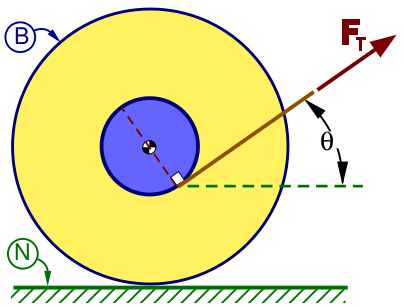
\includegraphics[height=5.5cm]{spool.png}
\isolatedBuildFooter